\section{Theorie}
\label{sec:Theorie}

Nach dem $\alpha$- oder $\beta$-Zerfall eines instabilen Nuklids kommt es vor, dass der neu entstehende Kern in einem angeregten Zustand ist. Nach einer kurzen Zeit fällt er unter Aussendung eines $\gamma$-Quants in seinen Grundzustand zurück.

\subsection{Wechselwirkung von Gamma-Strahlung mit Materie}

Trifft ein solches $\gamma$-Quant auf Materie, dominieren drei Arten von Wechselwirkungen dabei für unterschiedliche Energien. Die Wahrscheinlichkeit für jede Art von Wechselwirkung lässt sich durch einen Wirkungsquerschnitt $\sigma$ beschreiben, der anschaulich darstellt, dass die eingestrahlten Projektilteilchen ($\gamma$-Quanten) auf ein ausgedehntes Ziel um ein Targetteilchen (Absorberatom) treffen.\\
Die Wahrscheinlichkeit $\diff W$, dass ein Teilchen von dem Absorber eingefangen wird, lässt sich mit der Absorberschichtdicke $dx$ und der Anzahl der Elektronen pro Volumeneinheit $n$ ausdrücken durch:
\begin{equation}
\diff W = n \sigma \diff x\text{.}
\end{equation}
Bei $N$ Quanten, die auf den infinitesimal dicken Absorber auftreffen, folgt für die Zahl der absorbierten Teilchen:
\begin{align*}
\diff N = -N  \diff W =-n N \sigma \diff x\text{.}
\end{align*}
Daraus ergeben sich für einen Absorber der Dicke $D$ die Anzahl der wechselgewirkten Quanten $N_2(D)$ und die Anzahl der noch verbliebenen Quanten $N(D)$:
\begin{align}
N(D) 	&= N_0 \exp(-n \sigma D) \text{,}\\ 
N_2(D) 	&= N_0 (1 - \exp(-n \sigma D))\text{.}\label{eq:Nd}
\end{align}
Die Anzahl der auf den Absorber treffenden Quanten wird mit $N_0$ bezeichnet. Die Konstante $ \mu = n \sigma$ wird auch als Extinktionskoeffizient bezeichnet und ihr Kehrwert liefert die mittlere Reichweite der Quanten im Absorber. In Abbildung \ref{fig:Wirkungsquerschnitt} sind die Extinktionskoeffizienten $\mu=n\sigma$ der nachfolgend beschriebenen Wirkungsquerschnitte in Abhängigkeit von der Energie der $\gamma$-Quanten zu sehen.

\begin{figure}
	\centering
	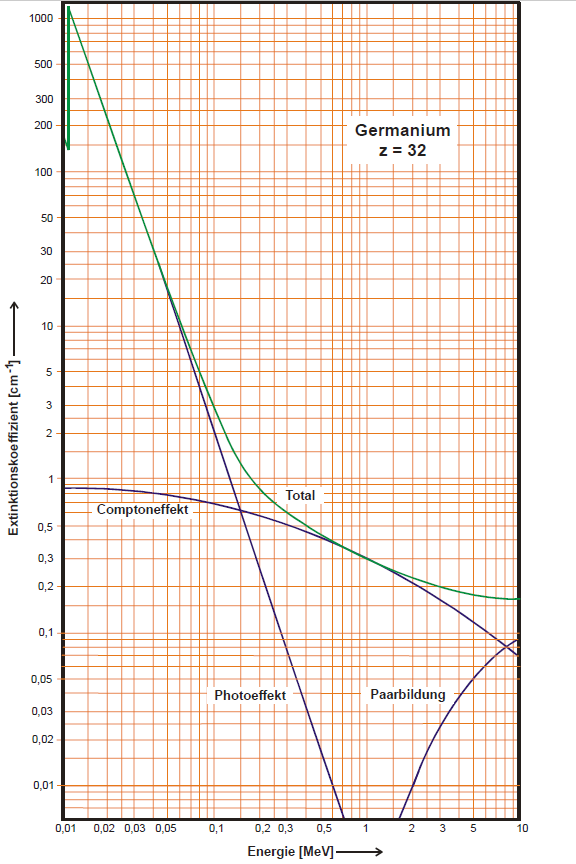
\includegraphics[width=\linewidth-70pt,height=\textheight-70pt,keepaspectratio]{content/images/sigma.png}
	\caption{Energieabhängigkeit des Extinktionskoeffizienten $\mu$ für Germanium getrennt nach den verschiedenen Wechselwirkungsmechanismen \cite{V18}.}
	\label{fig:Wirkungsquerschnitt}
\end{figure}

\subsubsection{Der Photoeffekt}

Beim Photoeffekt trifft ein $\gamma$-Quant auf ein Hüllenelektron und schlägt dieses aus der Bindung des Kerns. Das $\gamma$-Quant, das bei diesem Prozess vollständig absorbiert wird, muss dafür mindestens die Bindungsenergie $E_.B$ besitzen, sodass gilt:
\[
E_.{\gamma}>E_.B\text{.}
\]
Findet die Reaktion in einer inneren Schale statt, fällt ein Elektron aus einem höheren Zustand unter Aussendung eines charakteristischen Röntgenquants, welches im Medium verbleibt, in das freigewordene Energieniveau. Somit kann angenommen werden, dass die vollständige Energie des $\gamma$-Quants deponiert wird, was bei einer Messung des Energiespektrums zu einem scharfen Peak führt.
Für den Wirkungsquerschnitt gilt dabei mit der Kernladungszahl $Z$ des Absorbers:
\[
\sigma_.{Ph}\propto\frac{Z^{\alpha}}{E^{\delta}_.{\gamma}}
\]
Es gilt $4 < \alpha < 5$.  Der Exponent $\delta$ ist abhängig von der Photonenenergie. Für natürlich vorkommende $\gamma$-Strahlung gilt $\delta\approx \num{3.5}$, für Energien $E_.{\gamma}\geq \SI{5}{\mega\electronvolt}$ sinkt er auf $\delta\approx 1$.
Der Wirkungsquerschnitt steigt außerdem immer sprunghaft an, wenn $E_.{\gamma}$ einen Wert erreicht, der ausreicht, um ein Elektron aus dem Atom herauszulösen. Die übrige Energie des $\gamma$-Quants wird vom Elektronen als kinetische Energie aufgenommen.

\subsubsection{Der Compton-Effekt}

Der Compton-Effekt beschreibt die elastische Streuung eines $\gamma$-Quants an einem als in Ruhe angenommenen Hüllenelektron. Das $\gamma$-Quant gibt dabei nur einen Teil der Energie ab und fliegt danach mit veränderter Frequenz abgelenkt weiter. Eine schematische Darstellung davon ist in Abbildung \ref{fig:Compton} zu sehen.
Geschieht dieser Effekt an einem Elektron auf einem äußeren Energieniveau, so kann dieses aus der Bindung herausgeschlagen werden. Bei stärker gebundenen Elektronen verbleibt das Elektron im gebundenen Zustand.
Der Energieübertrag lässt sich in Abhängigkeit des Winkels des auslaufenden $\gamma$-Quants bezüglich der Einfallsrichtung schreiben.
Da Energie und Impuls erhalten sind, müssen die Gleichungen
\begin{align*}
h \nu + m_.0 c^2 &= h \nu '+ \gamma m_.0 c^2\\
\frac{h \nu}{c}&= \frac{h \nu '}{c}\cos(\psi_.{\gamma})+\gamma m_.0 v\cos(\psi_.e)\\
0&= \frac{h\nu '}{c}\sin(\psi_.{\gamma})+\gamma m_.0 v\sin(\psi_.e)
\end{align*}
erfüllt sein. Dabei ist $h$ das Plancksche Wirkungsquantum, $c$ die Lichtgeschwindigkeit, $\gamma$ der Lorentzfaktor, $\nu$ und $\nu '$ die Frequenz des $\gamma$-Quants vor und nach dem Compton-Effekt und $\psi_.{\gamma}$ und $\psi_.e$ die Winkel des auslaufenden $\gamma$-Quants und des Elektrons bezüglich der Einfallsrichtung des $\gamma$-Quants.
Umformen und Gleichsetzen ergibt für die Energie des einfallenden und des auslaufenden $\gamma$-Quants $E_.{\gamma}=h\nu$ und $E_.{\gamma}'=h\nu '$ mit \[\epsilon=\frac{E_.{\gamma}}{m_.0c^2}\] die Beziehung
\begin{equation}
E_.{\gamma}'= E_.{\gamma}\frac{1}{1+\epsilon\cdot\left(1-\cos(\psi_.{\gamma})\right)}\text{.}
\end{equation}
Die Energiedifferenz
\begin{equation}
E_.e=E_.{\gamma}-E_.{\gamma}' =\frac{\epsilon\cdot\left(1-\cos(\psi_.{\gamma})\right)}{1+\epsilon\cdot\left(1-\cos(\psi_.{\gamma})\right)}E_.{\gamma}
\end{equation}
ist somit die an das Elektron abgegebene Energie.
Für $\psi_.{\gamma}=\SI{180}{\degree}$ ist sie maximal und beträgt
\begin{equation}
E_.{e,max}=\frac{2\epsilon}{1+\epsilon}E_.{\gamma}\text{.}\label{eq:Emax}
\end{equation}
Dieser Wert ist kleiner als $E_.{\gamma}$. Somit wird nie die gesamte Energie des $\gamma$-Quants auf das Elektron übertragen. Im Energiespektrum äußert sich das durch ein breites Kontinuum an Energien, welches an der Compton-Kante bei
$E_.{deponiert}=E_.{e,max}$ vor dem Photopeak endet.
Der Wirkungsquerschnitt des Compton-Effekts lässt sich über die Formel von Klein und Nishina beschreiben als
\begin{equation}
\sigma_.{Co}=\frac{3}{4}\sigma_.{Th}\left(\frac{1+\epsilon}{\epsilon^2}\left[\frac{2+2\epsilon}{1+2\epsilon}-\frac{1}{\epsilon}\ln(1+2\epsilon)\right]+\frac{1}{2\epsilon}\ln(1+2\epsilon)-\frac{1+3\epsilon}{(1+2\epsilon)^2}\right)\text{.}\label{eq:sig_Co}
\end{equation}
Dabei bezeichnet 
\[
\sigma_.{Th}=\frac{8}{3}\pi\left(\frac{e_.0}{4\pi\varepsilon_.0c^2m_.e}\right)^2
\] 
den Thomson-Wirkungsquerschnitt, mit der Elementarladung $e_.0$, der Dielektrizitätskonstante $\varepsilon_.0$, der Lichtgeschwindigkeit im Vakuum $c$ und der Ruhemasse des Elektrons $m_.e$.
Der differentielle Wirkungsquerschnitt $\frac{.d\sigma}{.dE}$ lässt sich beschreiben durch:
\begin{equation}
\frac{\diff \sigma}{\diff E} =  \frac{\pi r_\text{e}^2}{m_0 c^2 \epsilon^2}\left(2+\left(\frac{E_\text{e'}}{E_\gamma - E_\text{e'}}\right)^2 \left[ \frac{1}{\epsilon^2} +\frac{E_\gamma - E_\text{e'}}{E_\gamma} - \frac{2(E_\gamma - E_\text{e'})}{\epsilon E_\gamma} \right]\right) \text{.}\label{eq:sigmadiff}
\end{equation}

\begin{figure}
	\centering
	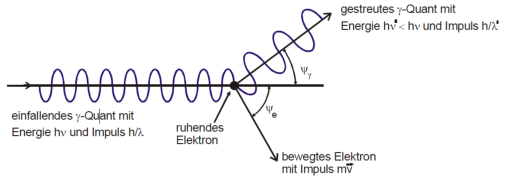
\includegraphics[width=\linewidth-50pt,height=\textheight-50pt,keepaspectratio]{content/images/Compton.pdf}
	\caption{Schematische Darstellung des Compton-Effekts \cite{V18}.}
	\label{fig:Compton}
\end{figure}

\subsubsection{Paarerzeugung}

Eine weitere Möglichkeit ist, dass sich das $\gamma$-Quant im Coulombfeld eines Kerns in ein Elektron und ein Positron aufspaltet. Auf Grund der Impulserhaltung muss es einen Stoßpartner geben. Ist dieser ein Atomkern, so ist die zusätzlich benötigte Rückstoßenergie 
\[
E_.r=\frac{p^2}{2M}
\]
mit der Atommasse $M$ gering, sodass die Energie des $\gamma$-Quants nur die Ruheenergie von Elektron und Positron übersteigen muss:
\[
E_.{\gamma}>2m_.0c^2\text{.}
\]
Ist der Stoßpartner ein Hüllenelektron, muss die Atommasse durch die Elektronenmasse ersetzt werden, wodurch $E_.R$ wesentlich größer ist und nicht mehr vernachlässigt werden kann.
In diesem Fall muss für die Energie des $\gamma$-Quants gelten:
\[
E_.{\gamma}>4m_.0c^2\text{.}
\]
Da Elektron und Positron dieselbe Masse besitzen, wird die verbleibende Energie gleichmäßig aufgeteilt.
Während das Elektron im Detektor durch Spannung abgesaugt wird, kann das Positron mit einem vorhandenen Hüllenelektron wieder zu zwei Photonen annihilieren.
Da diese den Detektor verlassen können ohne zu wechselwirken, können im Energiespektrum nicht nur eine Linie bei $E_.{\gamma}$, sondern auch Linien bei $E_.{\gamma}-m_.0c^2$ und bei $E_.{\gamma}-2m_.0c^2$ beobachtet werden.\\
Der Wirkungsquerschnitt ist abhängig davon, wo im Coulombfeld der Prozess stattfindet, da in den äußeren Schalen Abschirmungseffekte durch die Hüllenelektronen auftreten.
Der wichtigste Fall für die $\gamma$-Spektroskopie ist die Paarbildung in Kernnähe.
Hier gilt für den Wirkungsquerschnitt bei Energien $\SI{10}{MeV}<E_.{\gamma}<\SI{25}{MeV}$ näherungsweise mit der Sommerfeldschen Feinstrukturkonstante $\alpha$
\begin{equation}
\sigma_.P=\alpha r^2_.eZ^2\left(\frac{28}{9}\ln(2\epsilon)-\frac{218}{27}\right)\text{.}\label{eq:s_P}
\end{equation}

\subsection{Der Reinst-Germanium-Detektor}

\subsubsection{Aufbau und Voraussetzungen}

Der Germanium-Detektor ist ein Halbleiterdetektor. Er besteht aus einem n- und einem p-dotierten Bereich. Am Übergang diffundieren auf Grund thermischer Energie bei endlicher Temperatur einzelne Elektronen und Löcher in die jeweils andere Schicht und rekombinieren dort, sodass eine Ladungsträger verarmte Zone entsteht. Die Raumladungen der Donatoren in der n-Schicht und der Akzeptoren in der p-Schicht erzeugen eine Potentialdifferenz $U_.D$, die der Diffusion entgegenwirkt.
Durch eine asymmetrische Dotierung und das Anlegen einer Spannung $U$ lässt sich die Verarmungszone wesentlich verbreitern.
Für den Teil der Verarmungszone, der in der n- bzw. p-Schicht liegt, gilt
\begin{align*}
d^2_.n&=\frac{2\varepsilon_.r\varepsilon_.0}{e_.0}\left(U_.D+U\right)\frac{n_.A}{n_.D\left(n_.A+n_.D\right)},\\
d^2_.p&=d^2_.n\frac{n^2_.D}{n^2_.A},
\end{align*}
mit den Dielektrizitätskonstanten $\varepsilon_.r$ und $\varepsilon_.0$, der Elementarladung $e_.0$ und der Akzeptoren- und Donatorendichte $n_.A$ und $n_.D$.
Für $n_.D>>n_.A$ ist die Breite der Verarmungszone gegeben durch
\begin{equation}
d=d_.n+d_.p\approx d_.p\approx\sqrt{\frac{2\varepsilon_.r\varepsilon_.0}{e_.0}\left(U_.D+U\right)\frac{1}{n_.A}}\text{.}
\end{equation}
Eine möglichst geringe p-Dotierung führt somit zu einer Verbreiterung der ladungsträgerarmen Zone, ebenso wie eine Erhöhung der angelegten Spannung. Durch thermische Energie entstandene Ladungsträger in der Verarmungszone können allerdings durch $U$ beschleunigt werden. Es kommt zu Avalanche-Durchbrüchen und damit zu Signalen, auch wenn nichts detektiert wird.
Um derartige Effekte zu vermeiden, wird der Detektor auf eine Temperatur von $\SI{77}{\kelvin}$ abgekühlt.
Der hier verwendete Detektor ist ein koaxialer Reinst-Germanium-Detektor. Zur n-Dotierung wird die Oberfläche des Ge-Kristalls mit Lithium bedampft und der Pluspol der Spannung angeschlossen.
Eine koaxiale Bohrung im Kristall wird mit Gold bedampft und der Minuspol der Spannung angeschlossen. Da der Kristall auf Grund seiner Reinheit selbst eine sehr geringe Akzeptorendichte von $n_.A=\SI{e10}{\per\cm^3}$ aufweist, kommt es zur Ausbildung der Verarmungszone. Weiterhin ist der Detektor zur thermischen Isolation von einer Aluminium-Haube umgeben. Das führt dazu, dass nur Photonen detektiert werden können, die genügend Energie besitzen, um diese Aluminium-Schicht und die Lithium-Schicht auf der Kristalloberfläche zu durchdringen. Der Querschnitt eines solchen Detektors ist in Abbildung \ref{fig:Det} zu sehen.
\begin{figure}
	\centering
	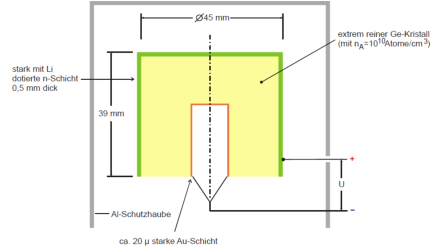
\includegraphics[width=\linewidth-50pt,height=\textheight-50pt,keepaspectratio]{content/images/Detektor.pdf}
	\caption{Querschnitt eines Germanium-Detektors mit Al-Ummantelung \cite{V18}.}
	\label{fig:Det}
\end{figure}

\subsubsection{Funktionsweise}

Trifft ein geladenes Teilchen oder ein Photon auf die Verarmungszone, deponiert es dort Energie. Dadurch können einge Elektronen die Energielücke zwischen Valenz- und Leitungsband überspringen und hinterlassen im Valenzband ein ebenfalls bewegliches Loch, sodass Elektronen-Loch-Paare entstehen. Diese Bandlücke beträgt für Germanium $\SI{0,67}{\electronvolt}$, jedoch wird für die Erzeugung von Elektronen-Loch-Paaren eine Energie von $E_.{ELP}=\SI{2,9}{\electronvolt}$\cite{V18} benötigt, da dieser Prozess nur unter Anregung von Phononen geschieht. Durch die angelegte Spannung werden die Elektronen am Plus- und die Löcher am Minuspol gesammelt, bevor sie rekombinieren, was zu einem messbaren Ladungsimpuls führt, dessen Betrag ein Maß für die Anzahl der Elektronen-Loch-Paare und damit für die deponierte Energie ist.

\subsubsection{Auflösungsvermögen und Effizienz}
\label{subsubsec:Effizienz}

Im vom Detektor aufgezeichneten Spektrum eines $\gamma$-Strahlers können zwei Spektrallinien nur dann unterschieden werden, wenn ihre Mittelwerte mindestens um die Halbwertsbreite $\Delta E_.{1/2}$ entfernt voneinander liegen.
Wenn $n$ die Anzahl der erzeugten Elektronen-Loch-Paare ist und $\bar{n}=\frac{E_.{\gamma}}{E_.{ELP}}$ würde sich bei einer von den Phononen unkorrelierten Verteilung die Standardabweichung berechnen zu
\[
\sigma=\sqrt{\bar{n}}\text{.}
\]
Die Anregung der Phononen wird durch den Fanofaktor $F$ berücksichtigt. Für Germanium ist $F\approx 0,1$.
Damit ist 
\[
\sigma=\sqrt{F\bar{n}}\approx\sqrt{0,1\frac{E_.{\gamma}}{E_.{ELP}}}\text{.}\label{eq:sig}
\]
Da $n>>1$ lässt sich die Poisson-Verteilung der Linien durch eine Gauß-Verteilung approximieren, sodass
\begin{equation}
\Delta E_.{1/2}=\sqrt{8\ln(2)}\frac{\sigma}{\bar{n}}E_.{\gamma}\approx 0,74\sqrt{E_.{\gamma}E_.{ELP}}\text{.}\label{eq:dE}
\end{equation}
Verschlechtert wird die Auflösung durch das thermische Rauschen, dass durch die angelegte Saugspannung vergrößert wird, jedoch durch Abkühlen des Detektors erheblich verringert werden kann. Ein weiterer Faktor ist, dass die Sammlung der Ladungsträger durch Feldinhomogenitäten behindert wird, was durch eine Erhöhung von $U$ verringert werden kann. Unabhängig vom Detektor selbst verschlechtert auch das Rauschen des zur Signalweiterleitung angeschlossenen Verstärkers die Energieauflösung. Da alle diese Vorgänge unkorreliert ablaufen, addieren sich ihre Halbwertsbreiten quadratisch zu
\begin{equation}
H_.{Ges}=\Delta E^2_.{1/2} + H^2_.{the} + H^2_.{inh} + H^2_.{Ver}\text{.}\label{eq:HGes}
\end{equation}
\\
Die Effizienz $Q$ gibt die Abhängigkeit der Nachweiswahrscheinlichkeit von der Energie der zu messenden $\gamma$-Quanten an.
Sie lässt sich berechnen über
\begin{equation}
Q=\frac{Z}{W A}\frac{4\pi}{\Omega}\frac{1}{t}\text{.}\label{eq:Q}
\end{equation}
$W$ ist die vom Strahler abhängige Emissionswahrscheinlichkeit für eine bestimmte Spektrallinie, $Z$ ist der Inhalt des Peaks und $t$ ist die Messzeit.
Die Aktivität $A$ lässt sich aus der Aktivität zum Herstellungszeitpunkt und der seitdem vergangen Zeit berechnen:
\begin{equation}
A(t) = A_0\cdot \exp\left(\frac{-\ln(2)t}{\tau_{1/2}}\right)\text{,}\label{eq:A} 
\end{equation}
mit der Halbwertszeit $\tau_{1/2}$.
Für den Raumwinkel $\Omega$, unter dem die Probe vom Detektor gesehen wird, gilt näherungsweise:
\begin{equation}
\frac{\Omega}{4\pi} = \frac{1}{2}\left(1-\frac{a}{\sqrt{a^2+r^2}}\right)\text{,}\label{eq:Omega}
\end{equation}
mit dem Radius $r$ des Detektors und dem Abstand $a$ der Probe zum Detektor.\newpage
\noindent Das Spektrum eines monochromatischen $\gamma$-Strahlers ist in Abbildung \ref{fig:Spektrum} zu sehen.
Der Rückstreupeak im Compton-Kontinuum, welches an der Compton-Kante endet entsteht dadurch, dass Photonen bereits außerhalb des Detektors streuen und erst in diesen eindringen, nachdem sie bereits einen Teil ihrer Energie abgegeben haben. Der Photo-Peak liegt, abgeschnitten vom Kontinuum, in einem höheren Energiebereich.
\begin{figure}
	\centering
	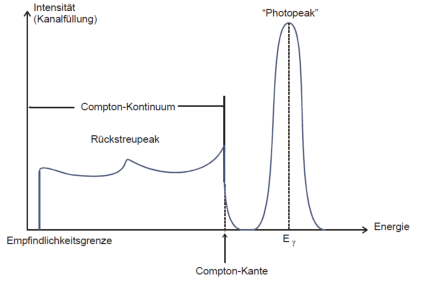
\includegraphics[width=\linewidth-70pt,height=\textheight-70pt,keepaspectratio]{content/images/Spektrum.pdf}
	\caption{Spektrum eines monochromatischen $\gamma$-Strahlers \cite{V18}.}
	\label{fig:Spektrum}
\end{figure}

